\chapter{Introduction}
\begin{chapabstract}

Intro intro intro intro.

\end{chapabstract}
\section{Background}

The low-frequency radio emission from star-forming galaxies has been studied for many years.
In this paper, we use the term ``Low frequency'' as the frequency less than a few GHz.
The importance of this emission increased after the global log-linear correlation with infrared (IR) had been found.
This correlation was discovered by \citet{Helou1985} using integrated far-infrared (FIR;\@$60\,\micron$ and $100\,\micron$) and $1.4\GHz$ radio luminosities in star-forming galaxies, and called the IR-Radio Correlation (IRC).
\citet{Condon1991a,Yun2001a, Bell2003} have examined this global correlation using a different sample set and found it holds the tightness across more than three orders of magnitude.
Recently, the low-frequency survey at around $100\MHz$ was operated by the LOw Frequency Array (LOFAR;~\citealt{VanHaarlem2013}) and the Murchison Widefield Array (MWA;~\citealt{Tingay2013a}).
With the advent of these telescopes, \citet{CalistroRivera2017a, Read2018, Wang2019} extend the IRC study to at an order of magnitude lower frequency and find IRC is held at not only $1.4\GHz$ but $\sim 100\MHz$.

Thanks to this correlation, we can regard the low frequency emission as a SFR indicator because IR luminosity is emitted by heated dust grains in a galaxy and can measure the SFR\@.
Since the low-frequency emission is not affected by the dust extinction \citep{Yun2001a, Murphy2011} and it will be observed from a distant galaxies by the future extended survey, we anticipate its usefulness and need a further investigation of the relation between the radio and IR luminosities, especially its frequency dependence.
However, the spatially-resolved studies show that a star-forming galaxy emits the radio emission whose spectral index depends on the galaxy region \citep{Kapinska2017a, For2018a, Heesen2019}.
This means that the radio emission is sensitive to the local density environment of the ISM and it is not guaranteed a simple frequency dependence of the global relation between the integrated radio and IR luminosities.

The integrated radio emission in star-forming galaxies across $100\MHz$ to $1.4\GHz$ is supposed to compose of a few percent to $10\%$ free-free and the synchrotron radiations \citep{Condon1992a}.
Each radiation is emitted by electrons interacted with the electric field of ions in the \ih~region or the magnetic field in a galaxy.
For emitting the synchrotron radiation, an electron needs to be accelerated to the light speed by the supernova remnant.
While the synchrotron emission is expected to be dominant at these low frequencies, previous studies find the sign of the free-free absorption and flatter or turnover spectral \citep{Schober2017, Chyzy2018}.
If the radio emission has a significant turnover among low frequencies, IRC does not have a simple frequency dependence and the radio emission is no longer useful as a SFR indicator.

In this study, we investigate nearby star-forming galaxies from the reference sample for ensuring the reliability of measuring the SFR from the low-frequency emission.
For examining the general trend, we use star-forming galaxy samples from Herschel Reference Survey (HRS;~\citealt{Boselli2010}) catalog which are supposed to represent the galaxy samples and the low-frequency emission from The GaLactic Extragalactic All-sky MWA (GLEAM;~\citealt{Hurley-Walker2017a}) Survey which observes the mJy scale radio emission from large areas with their 20 narrow bands.

This paper is organized as follows.
In Section~\ref{sec:sample}, we introduce our galaxy samples and the low-frequency emissions used in this study.
In Section~\ref{sec:Method}, we introduce the IR-Radio Correlation with the $\qn$ value defined for evaluating the correlation quantitatively. Here, we also mention the way to investigate its frequency dependence and derive the radio SFR\@.
In Section~\ref{sec:results}, we show our results about the frequency dependence of IRC and the consistency of the radio SFR\@.
In Section~\ref{sec:discussion}, we compare our results with previous studies.
Finally, we summarize our study in Section~\ref{sec:summary}.



%\bibliographystyle{mnras}
%%\bibliography{example} % if your bibtex file is called example.bib
%\bibliography{masterthesis}




%Reference Table \ref{tab:Table1}.  And blah blah blah.
%
%\begin{table}[t]
%\caption[TOC Table Description]{Caption.}
%	\centering
%	\begin{tabular}{lcc}
%		\hline
%        {\textbf{Setting}}                      & \multicolumn{2}{c}{\textbf{Mt C/y}} \\
%		                                                           &         Min          &     Max      \\ \hline
%		AAA                         &          40          &      66      \\
%		BBB                               &          14          &      66      \\
%		CCC                                       &          18          &      43      \\
%		DDD      &          4           &    $>$12     \\
%		EEE                                  &          0           &      47      \\
%		FFF                    & 1$ \times $10$^{-4}$ &      52      \\
%		GGG &          8           &      42      \\ \hline
%	\end{tabular}
%    \label{tab:Table1}
%\end{table}
%
%\section{Figures}
%Reference Figure~\ref{fig:Fig1}.
%
%\subsection{This is a subsection}
%\begin{figure}[t]
%	\centering
%	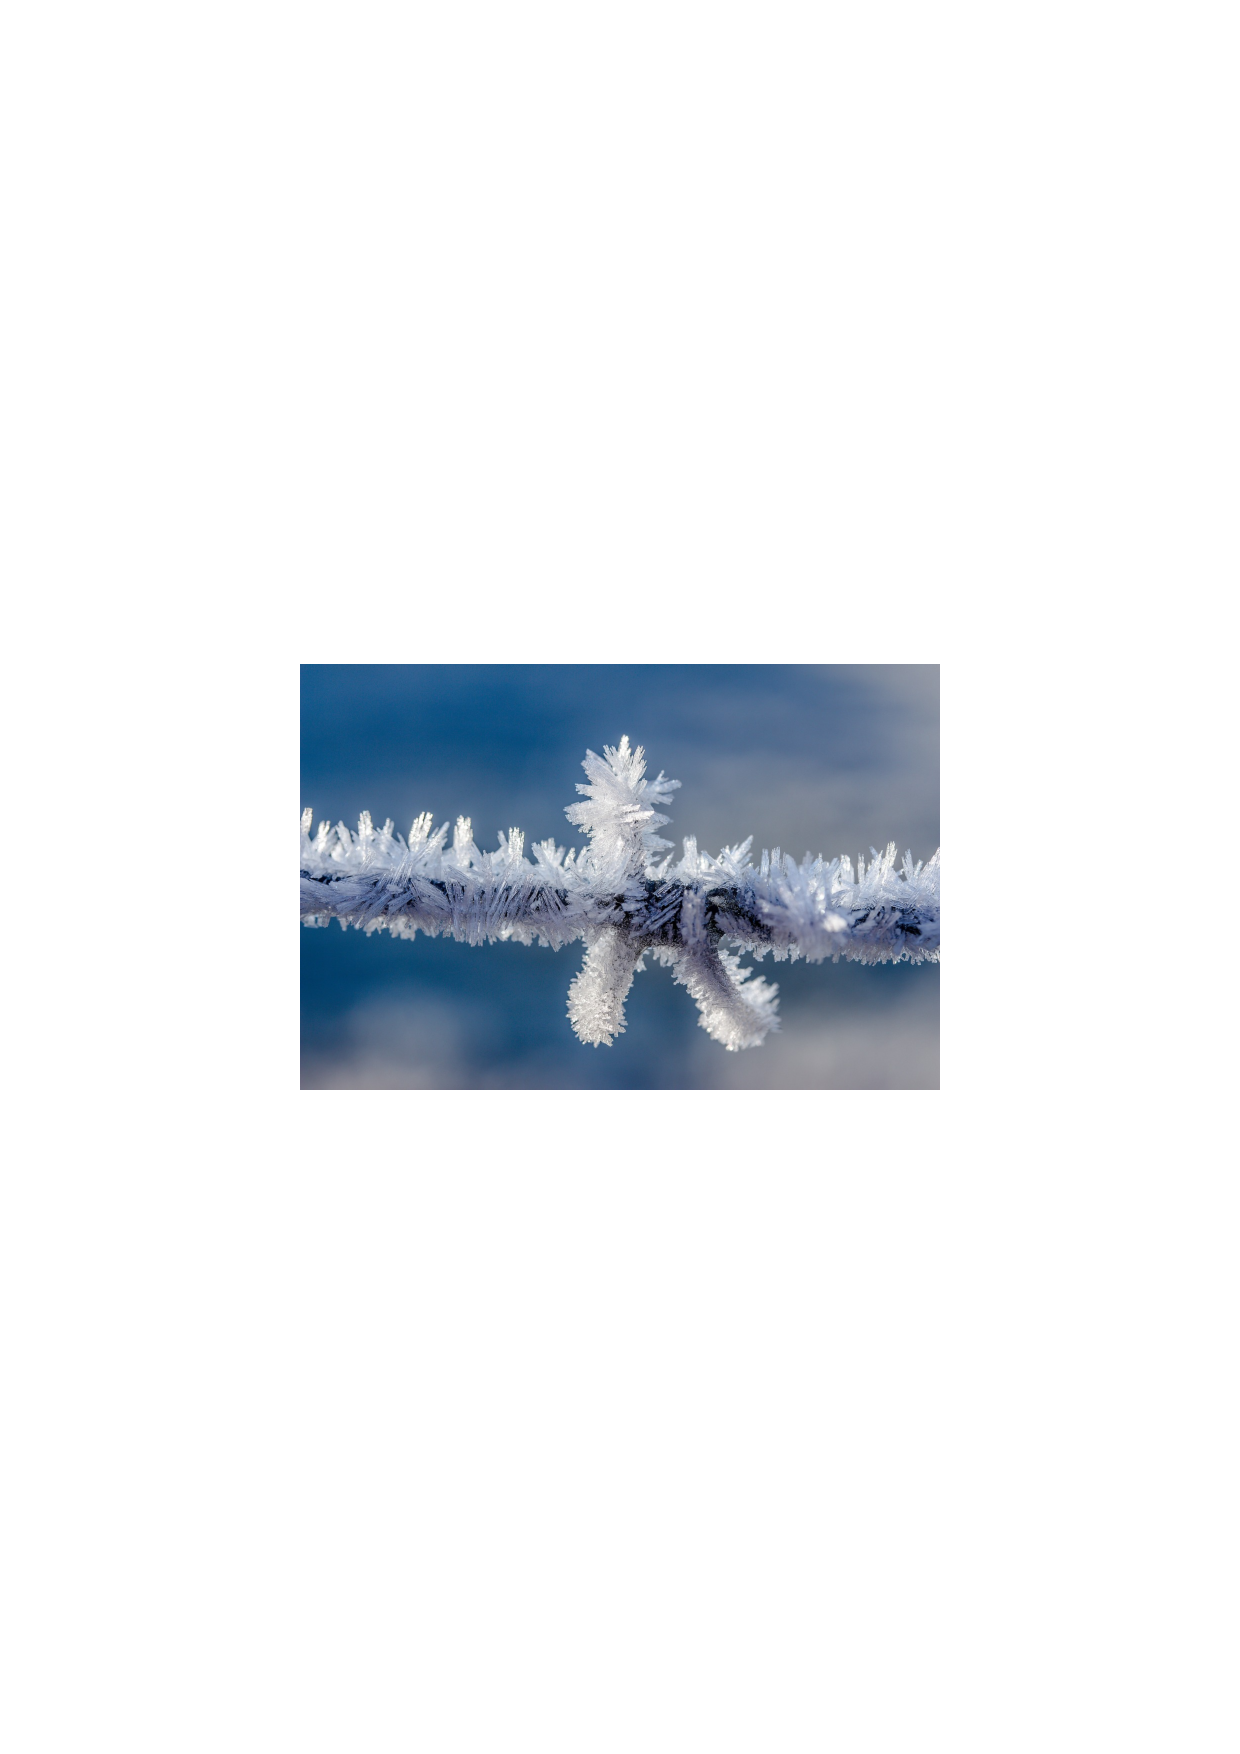
\includegraphics[width=.6\linewidth]{Chapter_1/Figs/Fig1.pdf}
%	\caption[TOC Figure Description]{Caption.}
%	\label{fig:Fig1}
%\end{figure}
%\subsubsection{This is a subsubsection}
%Citations are like \cite{goossens93,AbedonHymanThomas2003}.  Or maybe \cite{Abedon1994} said something.  Or \cite{Cerveny} which is an example of how to make a bib file that includes an author whose name begins with a non-English character and \cite{forgues96}: an example of referencing a Ph.D. thesis and yet more non-English characters.




%\bibliographystyle{abbrvnat}
%\bibliography{Chapter_1/ref1}
